\documentclass[12pt, a4paper]{article}

\usepackage[slovak]{babel}
\usepackage[utf8]{inputenc}
\usepackage[T1]{fontenc}
\usepackage{geometry}
\usepackage{hyperref}
\usepackage{setspace}
\usepackage{subcaption}
\usepackage{afterpage}
\usepackage{graphicx}
\usepackage{csquotes}
\usepackage{longtable}
\usepackage{placeins}
\usepackage{pdfpages}
\usepackage{listings}
\usepackage{expl3}

% Dots in TOC
\usepackage{tocloft}
\renewcommand{\cftsecleader}{\cftdotfill{\cftdotsep}}

\renewcommand{\ttdefault}{pcr}
\lstdefinestyle{cstyle}{
   language=C,
	basicstyle=\linespread{1.1}\ttfamily\footnotesize,
   numbers=left,
   numberstyle=\tiny,
   frame=single,
   tabsize=4,
   captionpos=b,
   breaklines=true,
   texcl=true,
	numbersep=8pt,
	framexleftmargin=15pt,
	xleftmargin=5ex,
   xrightmargin=3.4pt,
	morekeywords = {uint8_t,uint16_t,int16_t,uint32_t,int32_t,bool}
}
\renewcommand{\lstlistingname}{Zdrojový kód}


\setstretch{1.5}
\widowpenalty10000
\clubpenalty10000
\newsavebox\shield
\usepackage{titlesec}

\usepackage[style=iso-numeric,backend=biber]{biblatex}
\addbibresource{literature.bib}
%\AtBeginBibliography{\small}

\geometry{
	a4paper,
	top=2cm,
	left=3cm,
	right=2.5cm,
	bottom=2.5cm
}

\begin{document}
\begin{titlepage}
{\centering
   {\Large Slovenská technická univerzita v Bratislave}\par
   {\Large Fakulta informatiky a informačných technológií}\par
   \vspace{\medskipamount}
   \vfill
   \LARGE \textbf{Inteligentné osvetlenie pracovného stola} \\
   \vspace{0.7\bigskipamount}
   {\Large Semestrálny projekt}\par
   \vfill
}
\normalsize   
\begin{flushleft}
\textbf{Autor:} Bc. Miroslav Hájek \\
\textbf{Študijný program:} Inteligentné softvérové systémy \\
\textbf{Predmet:} Vnorené systémy \\
\textbf{Akademický rok:} 2022 / 2023 \\
\end{flushleft}
\end{titlepage}

\thispagestyle{empty}
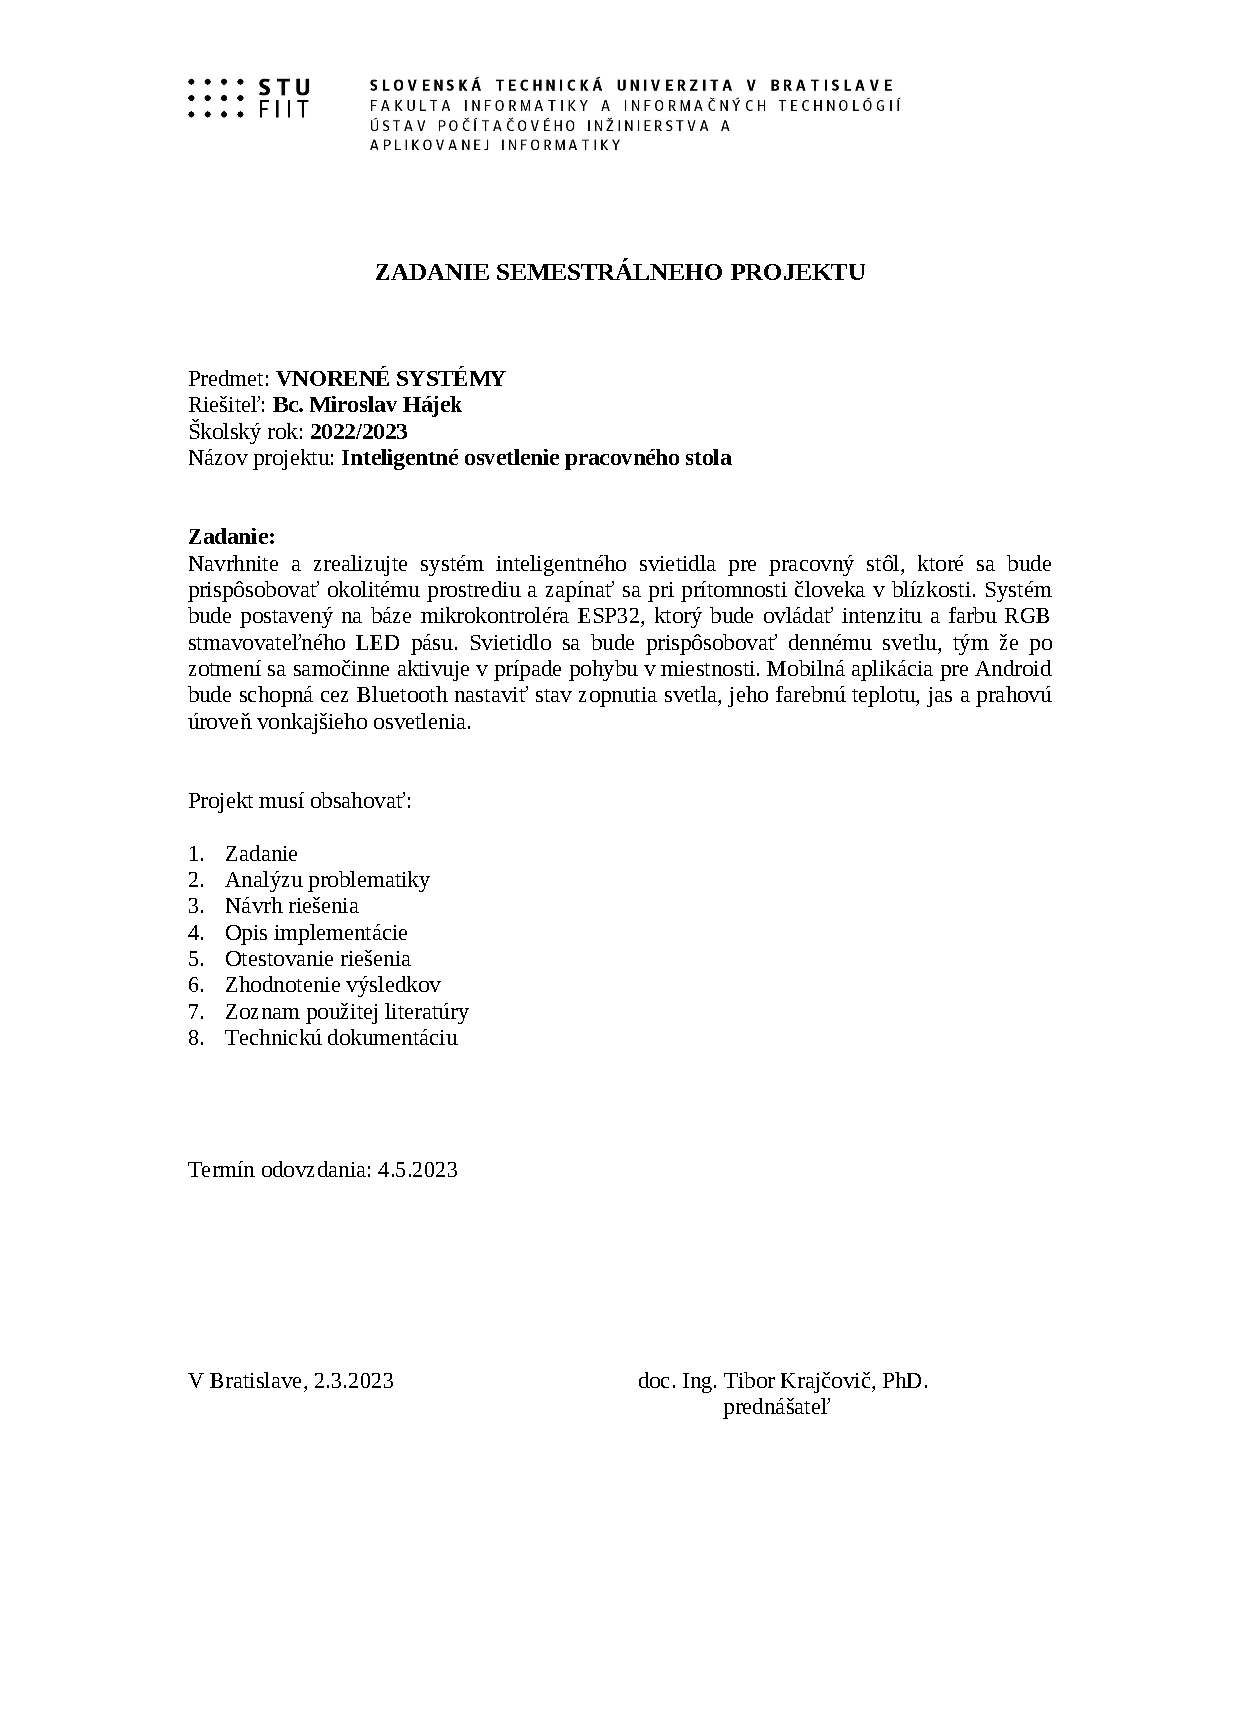
\includepdf[pages=-, scale=1]{zadanie}

\pagenumbering{gobble}
\tableofcontents
\newpage

\pagenumbering{arabic}
\setcounter{page}{1}

\section{Analýza problematiky}
Zariadenie na ovládanie svietidla sa má skladať z dvoch nezávislých integrovaných častí: riadiaca jednotka s firmvérom priamo regulujúca spínanie lampy podľa senzorov, a mobilná aplikácia na zmenu aktívnych nastavení svetla a detekcie pohybu komunikujúca cez Bluetooth. V sekcii popíšeme výber vhodných súčiastok a základné princípy ich fungovania.

\subsection{Špecifikácia požiadaviek}
Zo zadania vyplýva niekoľko funkcionálnych požiadaviek na systém:
\begin{itemize}
\itemsep0pt
\item Svietidlo rovnomerne osvetlí celý povrch pracovného stola.
\item Svietidlo sa zapne pri slabom osvetlení a súčasne detekcii pohybu v miestnosti.
\item Používateľ je schopný cez mobilnú aplikáciu vypnúť/zapnúť svetlo, nastaviť farebnú teplotu, jas a prahovú úroveň pre slabé osvetlenie.
\item Používateľské nastavenia svietidla sa zachovajú medzi zapnutiami zariadenia.
\item Vnorený systém kontroléra svetla je postavený na mikrokontroléri ESP32.
\item Mobilná aplikácia je určená na platformu Android a komunikuje cez Bluetooth.
\end{itemize}

\subsection{Riadiaca jednotka}
Mikrokontrolér \textbf{ESP32 WeMos Lolin D32} (Obr.~\ref{fig:esp32}) sme zvolili spomedzi ostatných bežne dostupných vývojových dosiek (ako sú Arduino, Raspberry Pi, STM32, BeagleBone a pod.) hlavne pre podporu pre viacerých štandardných mikroprocesorových rozhraní na rozličných pinoch. Doska je postavená na module \emph{ESP32-WROOM-32} \cite{noauthor_esp32-wroom-32_2023}, ktorý disponuje procesorom s frekvenciou 80~MHz (až do 240~MHz) a pamäťou 4~MB Flash a 520~kB SRAM príliš nelimitujúce rozhodnutia na účely prototypu.

Napájacie napätie dosky je 3,3~V, ale cez USB konektor môžeme pripojiť zdroj 5~V. ESP32 sa vyznačuje aj dobrou podporou od výrobcu v podobe SDK obsahujúce ovládače na všetky dostupné rozhrania pre periférie ESP-IDF \cite{noauthor_esp-idf_nodate}, ktorý tiež zahŕňa operačný systém reálneho času FreeRTOS.

\begin{figure}[h]
	\centering
	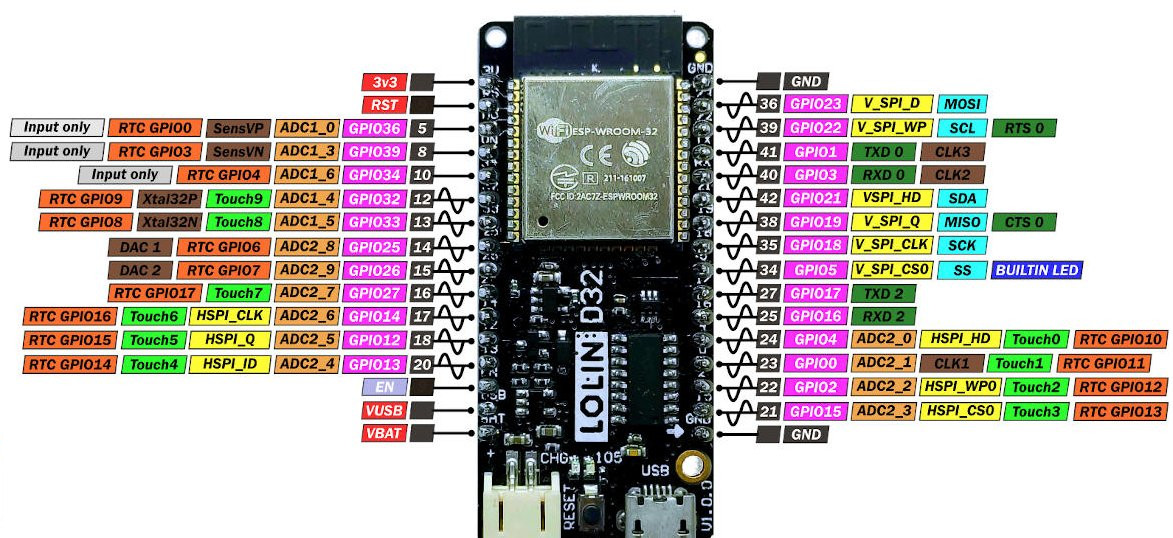
\includegraphics[width=\textwidth]{assets/esp32.jpg}
	\caption{Vývojová doska ESP32 WeMos Lolin D32 \cite{mischianti_esp32_2023}}
	\label{fig:esp32}
\end{figure}

ESP32 síce disponuje konektivitou na WiFi a Bluetooth, ale funkcie pre RFCOMM nie sú zatiaľ implementované, preto sa Bluetooth komunikácia musí realizovať externým \textbf{modulom HC-05} (Obr.~\ref{fig:hc-05}). Posielanie a príjem správ sa uskutočňuje cez \emph{UART} protokol, kde piny RXD a TXD musia byť na napäťových úrovniach 3,3 V, zatiaľ čo napájanie je v rozmedzí 3,6 - 6 V (zväčša 5 V). Baudová rýchlosť je predvolene určená na 9600.

Pin Enable slúži na prepnutie modulu do AT príkazového režimu (high úroveň), v ktorom je možné upraviť napr. baud. Pin State signalizuje stav Bluetooth pripojenia a je zároveň zapojený na indikačnú LED, ktorá sa môže nachádzať v 3 stavoch: (i) bliknutie raz za 2 sekundy - príkazový režim, (ii) blikanie 2-krát za 1 sekundu - pripojenie nadviazané, (iii) opakované blikanie - čakanie na pripojenie \cite{noauthor_hc-05_nodate}.

\begin{figure}[h]
	\centering
	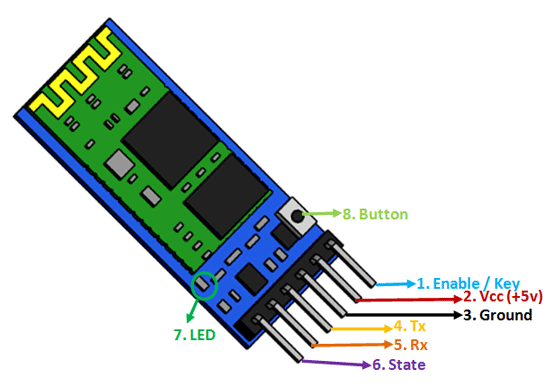
\includegraphics[width=0.5\textwidth]{assets/hc-05.png}
	\caption{Bluetooth modul HC-05 \cite{noauthor_hc-05_nodate}}
	\label{fig:hc-05}
\end{figure}

\subsection{Senzory a akčné členy}
Regulovateľné LED diódy v úlohe akčného členu musia reagovať na situáciu v okolitom prostredí, menovite detekciu pohybu človeka v miestnosti (cez infračervené čidlo) a intenzitu vonkajšieho osvetlenia (cez fotodiódu).

\subsubsection{RGB LED pásik}
Typ LED pásiku sa vyberá podľa rôznych kritérii ako sú účel použitia, či ide o dekoráciu alebo má slúžiť na osvetlenie miestnosti. Na základe toho prispôsobíme svetelný výkon, farbu, vodovzdornosť (stupeň ochrany krytom), rozmery, z čoho nakoniec vyplýva cieľové napätie najčastejšie 12~V, 24~V, 230~V.

Rozlišujeme pásiky podľa technológie produkcie teplotného odtieňu: jednofarebné, CCT - s dvoma typmi diód 2700~K a 6500~K a reguláciou medzi nimi, RGB - s štvorpinové LED diódami. Svietivosť pásiku ovplyvňuje príkon udávaný na meter, na nasvietenie napr. kuchynskej linky sa odporúča LED pásik s vyšším príkonom 12 - 20 W/m, tie je žiaduce namontovať na hliníkový podklad, z dôvodu chladenia. Ďalší faktor určujúci charakter svetla je rozloženie diód a ich počet na meter pásika \cite{123ledsk_ako_nodate}.

\begin{figure}[h]
\centering
\begin{subfigure}[b]{0.45\textwidth}
	\centering
	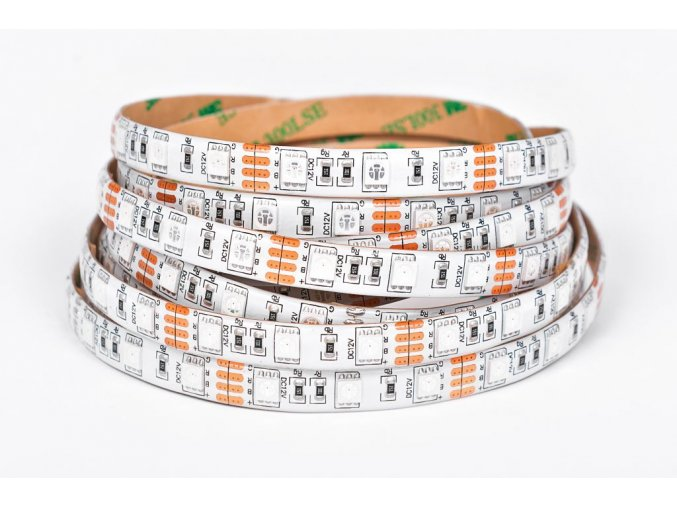
\includegraphics[width=\textwidth]{assets/rgb-led.jpg}
	\caption{LED pásik}
	\label{fig:rgb-led}
\end{subfigure}
\hfill
\begin{subfigure}[b]{0.5\textwidth}
	\centering
	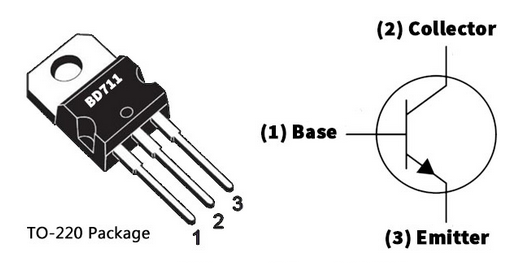
\includegraphics[width=\textwidth]{assets/bd711.png}
	\caption{NPN tranzistor BD711}
	\label{fig:bd-711}
\end{subfigure}
\caption{Akčné členy svietidla}
\end{figure}

Vhodný kandidát na interiérové osvetlenie stola sa ukazuje \textbf{RGB LED pásik} (Obr.~\ref{fig:rgb-led}) so samolepiacou fóliou 3M 300LSE bez krytia IP20, napätím zdroja 12~V, príkonom 14,4~W/m a hustotou diód 60~ks/m, ktorý vyprodukuje až 550~lm/m svetla \cite{123ledsk_rgb_nodate}. LED diódy na pásiku sú zapojenie tri do série so spoločnou anódou v 10 cm oddeliteľných úsekoch. Vetva pre červenú farbu má navyše zapojený do série 300~$\Omega$ SMD rezistor, ostatné vetvy majú zapojené 150~$\Omega$ rezistor.

Jednotlivé farebné kanály nemôžeme spínať a regulovať priamo s pinu mikroprocesoru, pretože nie je prítomné rovnaké napätie: 3,3~V voči 12~V, a nepostačuje ani maximálny prúd $I_{OL}$ = 28 mA. Dedikovaný tranzistor bude spínať prúd do 1,2 A ($I = 14,4W / 12V$), preto potrebujeme výkonovejšie tranzistory než z bežne používaného radu BC ($I_C < 100 mA$). \textbf{NPN tranzistor BD711} (Obr.~\ref{fig:bd-711}) dokáže spínať prúd až do 12 A \cite{noauthor_bd711_nodate}.

\begin{figure}[h]
\centering
\begin{subfigure}[b]{0.4\textwidth}
	\centering
	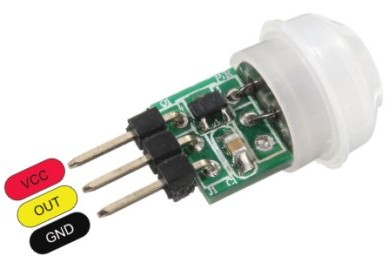
\includegraphics[width=\textwidth]{assets/pir-sb312.jpg}
	\caption{PIR senzor pohybu SB312}
	\label{fig:pir}
\end{subfigure}
\hfill
\begin{subfigure}[b]{0.4\textwidth}
	\centering
	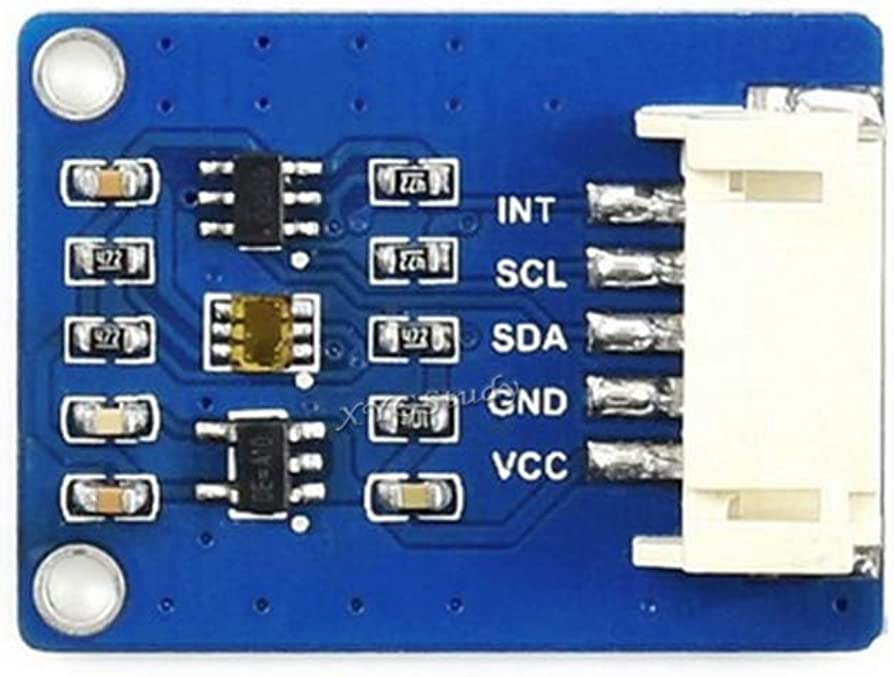
\includegraphics[width=\textwidth]{assets/tsl25911.jpg}
	\caption{Senzor osvetlenia TSL25911}
	\label{fig:light-sensor}
\end{subfigure}
\caption{Senzory s označením vývodov}
\end{figure}

\subsubsection{PIR pohybový senzor}
Na detekciu pohybu ľudí sa používajú infračervené PIR senzory líšiace sa veľkosťou, citlivosťou a nastaviteľnosťou úrovne detektora. Zlepšenie snímacích vlastností je docielené plastovou Fresnelovou šošovkou na senzore. \textbf{Olimex SB312} (Obr.~\ref{fig:pir})sa vyznačuje kompaktnosťou s rozmermi PCB: 10 x 8 mm. Disponuje uhlom snímacieho kužela do 100° s dosahom 3 - 5 metrov. Oneskorenie výstupu voči detegovanému pohybu je 2 sekundy a po rovnako dlhý čas drží výstupnú logickú úroveň v jednotke. Napájacie napätie senzora je 3,3~V \cite{olimex_pir-sb312_nodate}.

\subsubsection{Senzor okolitého osvetlenia}
Modul senzora osvetlenia Waveshare WS-17146 (Obr.~\ref{fig:light-sensor}) obsahuje obvod TSL25911FN, ktorý samostatne prerátava nameranú intenzitu svetla na fotodióde do luxov s použitím vzorca na aproximáciu ľudského videnia. Senzor pracuje na napätí 3,3~V aj 5~V a komunikuje cez I2C zbernicu do 400 kbit/s na adrese 0x29. Najdôležitejšie registre pre odčítanie aktuálnej hodnoty sú Control (0x01) a ALS Data (0x14 - 0x17) \cite{noauthor_tsl25911_nodate}.

\section{Návrh riešenia}
V časti návrhu uvažujeme ohľadom zapojenia hardvérových súčiastok z pohľadu napäťových úrovní aj riadiacich signálov v systéme. Spôsob čítania zo senzorov a ovládania ovplyvňujú ovládače adaptérov používané firmvérom a ich vzájomnú koordináciu. Voľbu nastavení, ktoré môže používateľ zmeniť je následne potrebné zahrnúť do prototypu obrazovky mobilnej aplikácie.

\subsection{Diagramy zapojenia}
Vnorený systém inteligentnej stolovej lampy vychádza z \textbf{blokovej schémy} na Obr. \ref{fig:block-diagram}. Zariadenie je napájané z elektrickej siete 230~V AC, ktoré napajací zdroj transformuje na 12~V DC priamo použiteľných pre LED pásik. Mikrokontrolér potrebuje napätie 3,3~V, ale USB konektor umožňuje pripojenie priamo na 5~V DC získaných z lineárneho regulátora napätia.

\begin{figure}[h]
	\centering
	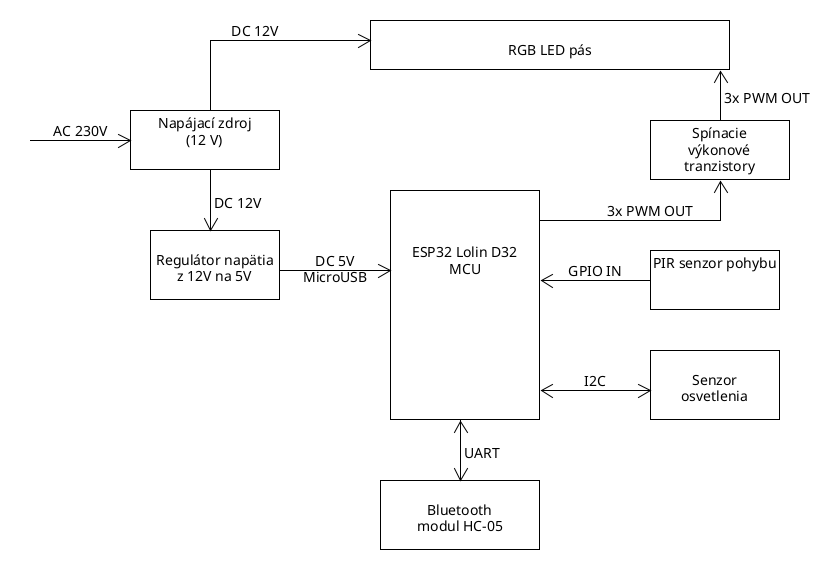
\includegraphics[width=\textwidth]{assets/block-diagram.png}
	\caption{Blokový diagram vnoreného systému inteligentného svietidla}
	\label{fig:block-diagram}
\end{figure}

Periférie komunikujú s ESP32 cez štandardné digitálne zbernice na napäťovej úrovni 3,3~V: UART pre Bluetooth modul, I2C pre senzor osvetlenia. Intenzita LED diód je regulovaná cez tri samostatné PWM kanály (pulzne-šírková modulácia) a senzor pohybu je pripojený ako vstup na GPIO pin.

\begin{figure}[h]
	\centering
	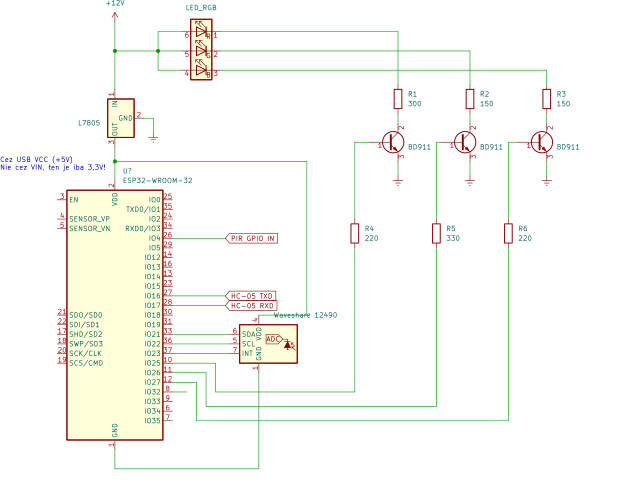
\includegraphics[width=0.8\textwidth]{assets/electrical-schematics.png}
	\caption{Schéma obvodu}
	\label{fig:electrical}
\end{figure}
Na schéme \ref{fig:electrical} je zakreslené zapojenie jednotlivých modulov na piny mikrokontroléra. Piny VCC a GND zo senzorov sú vedené na piny 3,3~V a GND na vývojovej doske ESP32. Bluetooth modul je pripojený priamo na 5~V z L7805. LED pásik už obsahuje rezistory pripojené na kolektory tranzistorov. Bázové rezistory sú zapojené ako prídavné súčiastky.

\subsection{Mobilná aplikácia}
Stav a aktuálne vlastnosti lampy sa budú nastavovať cez rozhranie mobilnej aplikácie určenej na platformu Android. Wireframe rozloženia tlačidiel a textových polí na vpisovanie čísel sa nachádza na Obr.~\ref{fig:app-wireframe}.
\begin{figure}[h]
	\centering
	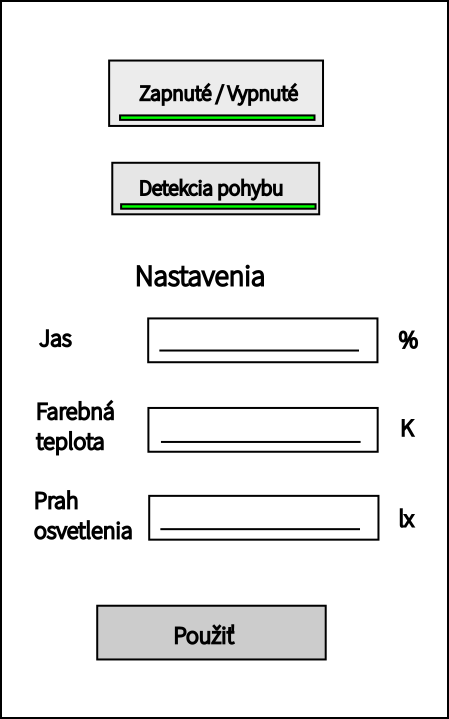
\includegraphics[width=0.28\textwidth]{assets/wireframe.png}
	\caption{Wireframe mobilnej aplikácie}
	\label{fig:app-wireframe}
\end{figure}

Funkcionality aplikácie budú dostupné až po úspešnom nadviazaní spojenia s modulom HC-05 cez Bluetooth. Pri pripojení na svietidlo si aplikácia načíta nastavenia uložené na mikrokontroléri do textových polí. Tlačidlo ,,Použiť'' umožní odoslať naraz všetky nastavenia z aplikácie. Na tlačidlách zapnutia svetla a detekcie pohybu, alebo vedľa nich, bude indikovaný aktuálny stav oznamovaný zo zariadenia pri akejkoľvek zmene.

\subsection{Spínanie svetla}
Svetlo sa môže v podstate nachádzať len v dvoch stavoch - zapnuté a vypnuté, aj keď charakter emitovaného svetla môže byť odlišný od situácie. Existuje však viacero scenárov na prepnutie stavu pri návrhu ktorých, je dôležité odstrániť konflikty. Nesmie nastať jav, že sa svetlo rozsvieti aktivovaním jedného pravidla a vzápätí sa zhasne uplatnením iného.
\begin{figure}[h]
   \centering
	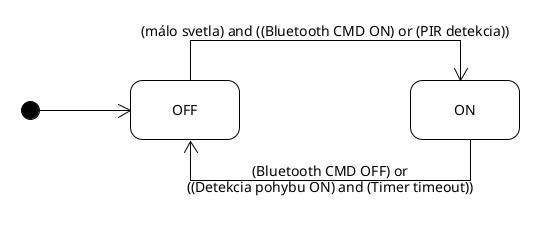
\includegraphics[width=0.7\textwidth]{assets/light-states.png}
	\caption{Stavový diagram spínania svietidla}
	\label{fig:state-diagram-switch}
\end{figure}

\begin{figure}[h]
   \centering
	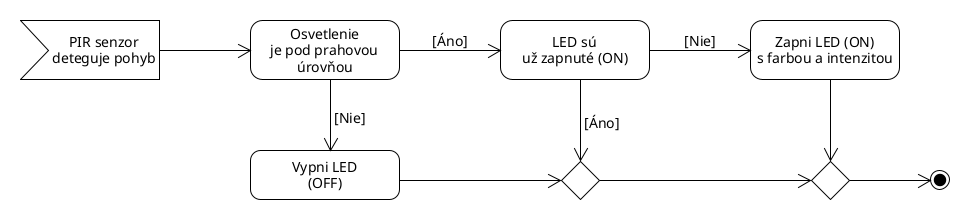
\includegraphics[width=\textwidth]{assets/pir-motion-detect.png}
	\caption{Zapnutie svietidla pri detekcii pohybu}
	\label{fig:pir-motion-detect}
\end{figure}

Pravidlá na prepnutie stavov svetla sú nasledovné (Obr.~\ref{fig:state-diagram-switch}):
\begin{itemize}
\item \textbf{Ak je OFF}: Okolité osvetlenie musí byť pod nastavenou prahovou úrovňou: lux~$\leq$~threshold, a súčasne bol zaslaný dopyt o zapnutie svetla, buď z mobilnej aplikácie alebo od pohybového senzora.
\item \textbf{Ak je ON}: Mobilná aplikácia poslala dopyt na vypnutie svetla alebo vypršal časovač od posledného dopytu na zapnutie (ten je aktívny vždy keď je spustená detekcia pohybu).
\end{itemize}
Postup zapnutia svetla pri detekcii pohybu je ilustrovaný na diagrame (Obr.~\ref{fig:pir-motion-detect}).

Okrem rozhodnutia na pokyn zapnutia LED pásika sa želaná farebná teplota a jas lampy musí prepočítať na striedu pulzno-šírkovej modulácie pre zložky farby v RGB:
\begin{enumerate}
\item \textbf{\emph{Farebná teplota [K]} → RGB}: prevod podľa algoritmu využívajúceho aproximáciu závislosti cez lineárnu regresiu medzi farebnou teplotou a energiou vyžiarenou čiernym telesom v danom farebnom kanály podľa CIE 1964 colour-matching funkcie. Regresný model používaný algoritmom je dostatočne presný s $R^2$ nad 0,987~\cite{helland_how_2012}.
\item \textbf{RGB → HSV}: konverzia na model HSV pre úpravu jasu výslednej farby svetla
\item \textbf{V ← \emph{Jas [lux]}}
\item\textbf{HSV→ RGB}
\item \textbf{PWM driver 8-bit výstup}: PWM kontroler má nastavené rozlíšenie presne na 8 bitov, čiže RGB trojica môže byť priamo nastavená do registra striedy výstupných kanálov.
\end{enumerate}

\section{Opis implementácie}
\textbf{Hardvérové súčiastky} vnoreného systému sú osadené na univerzálnom plošnom spoji (Obr.~\ref{fig:pcb}). Keďže sa jedná o prototyp sú komponenty podľa možností pripojené cez nespájkované prepojovacie kábliky alebo konektory, aby mohli byť jednoducho vymenené v prípade potreby. Na testovacie účely z dôvodu skladnosti bol využívaný jeden úsek LED pásiku, ale v prevádzke sa nahradí metrovou hliníkovou lištou s matným krytom (Obr.~\ref{fig:lamp-full}). Lišta bude prilepená obojstrannou páskou na poličku nad stolom.

\begin{figure}[h]
\centering
\begin{subfigure}[h]{0.48\textwidth}
	\centering
	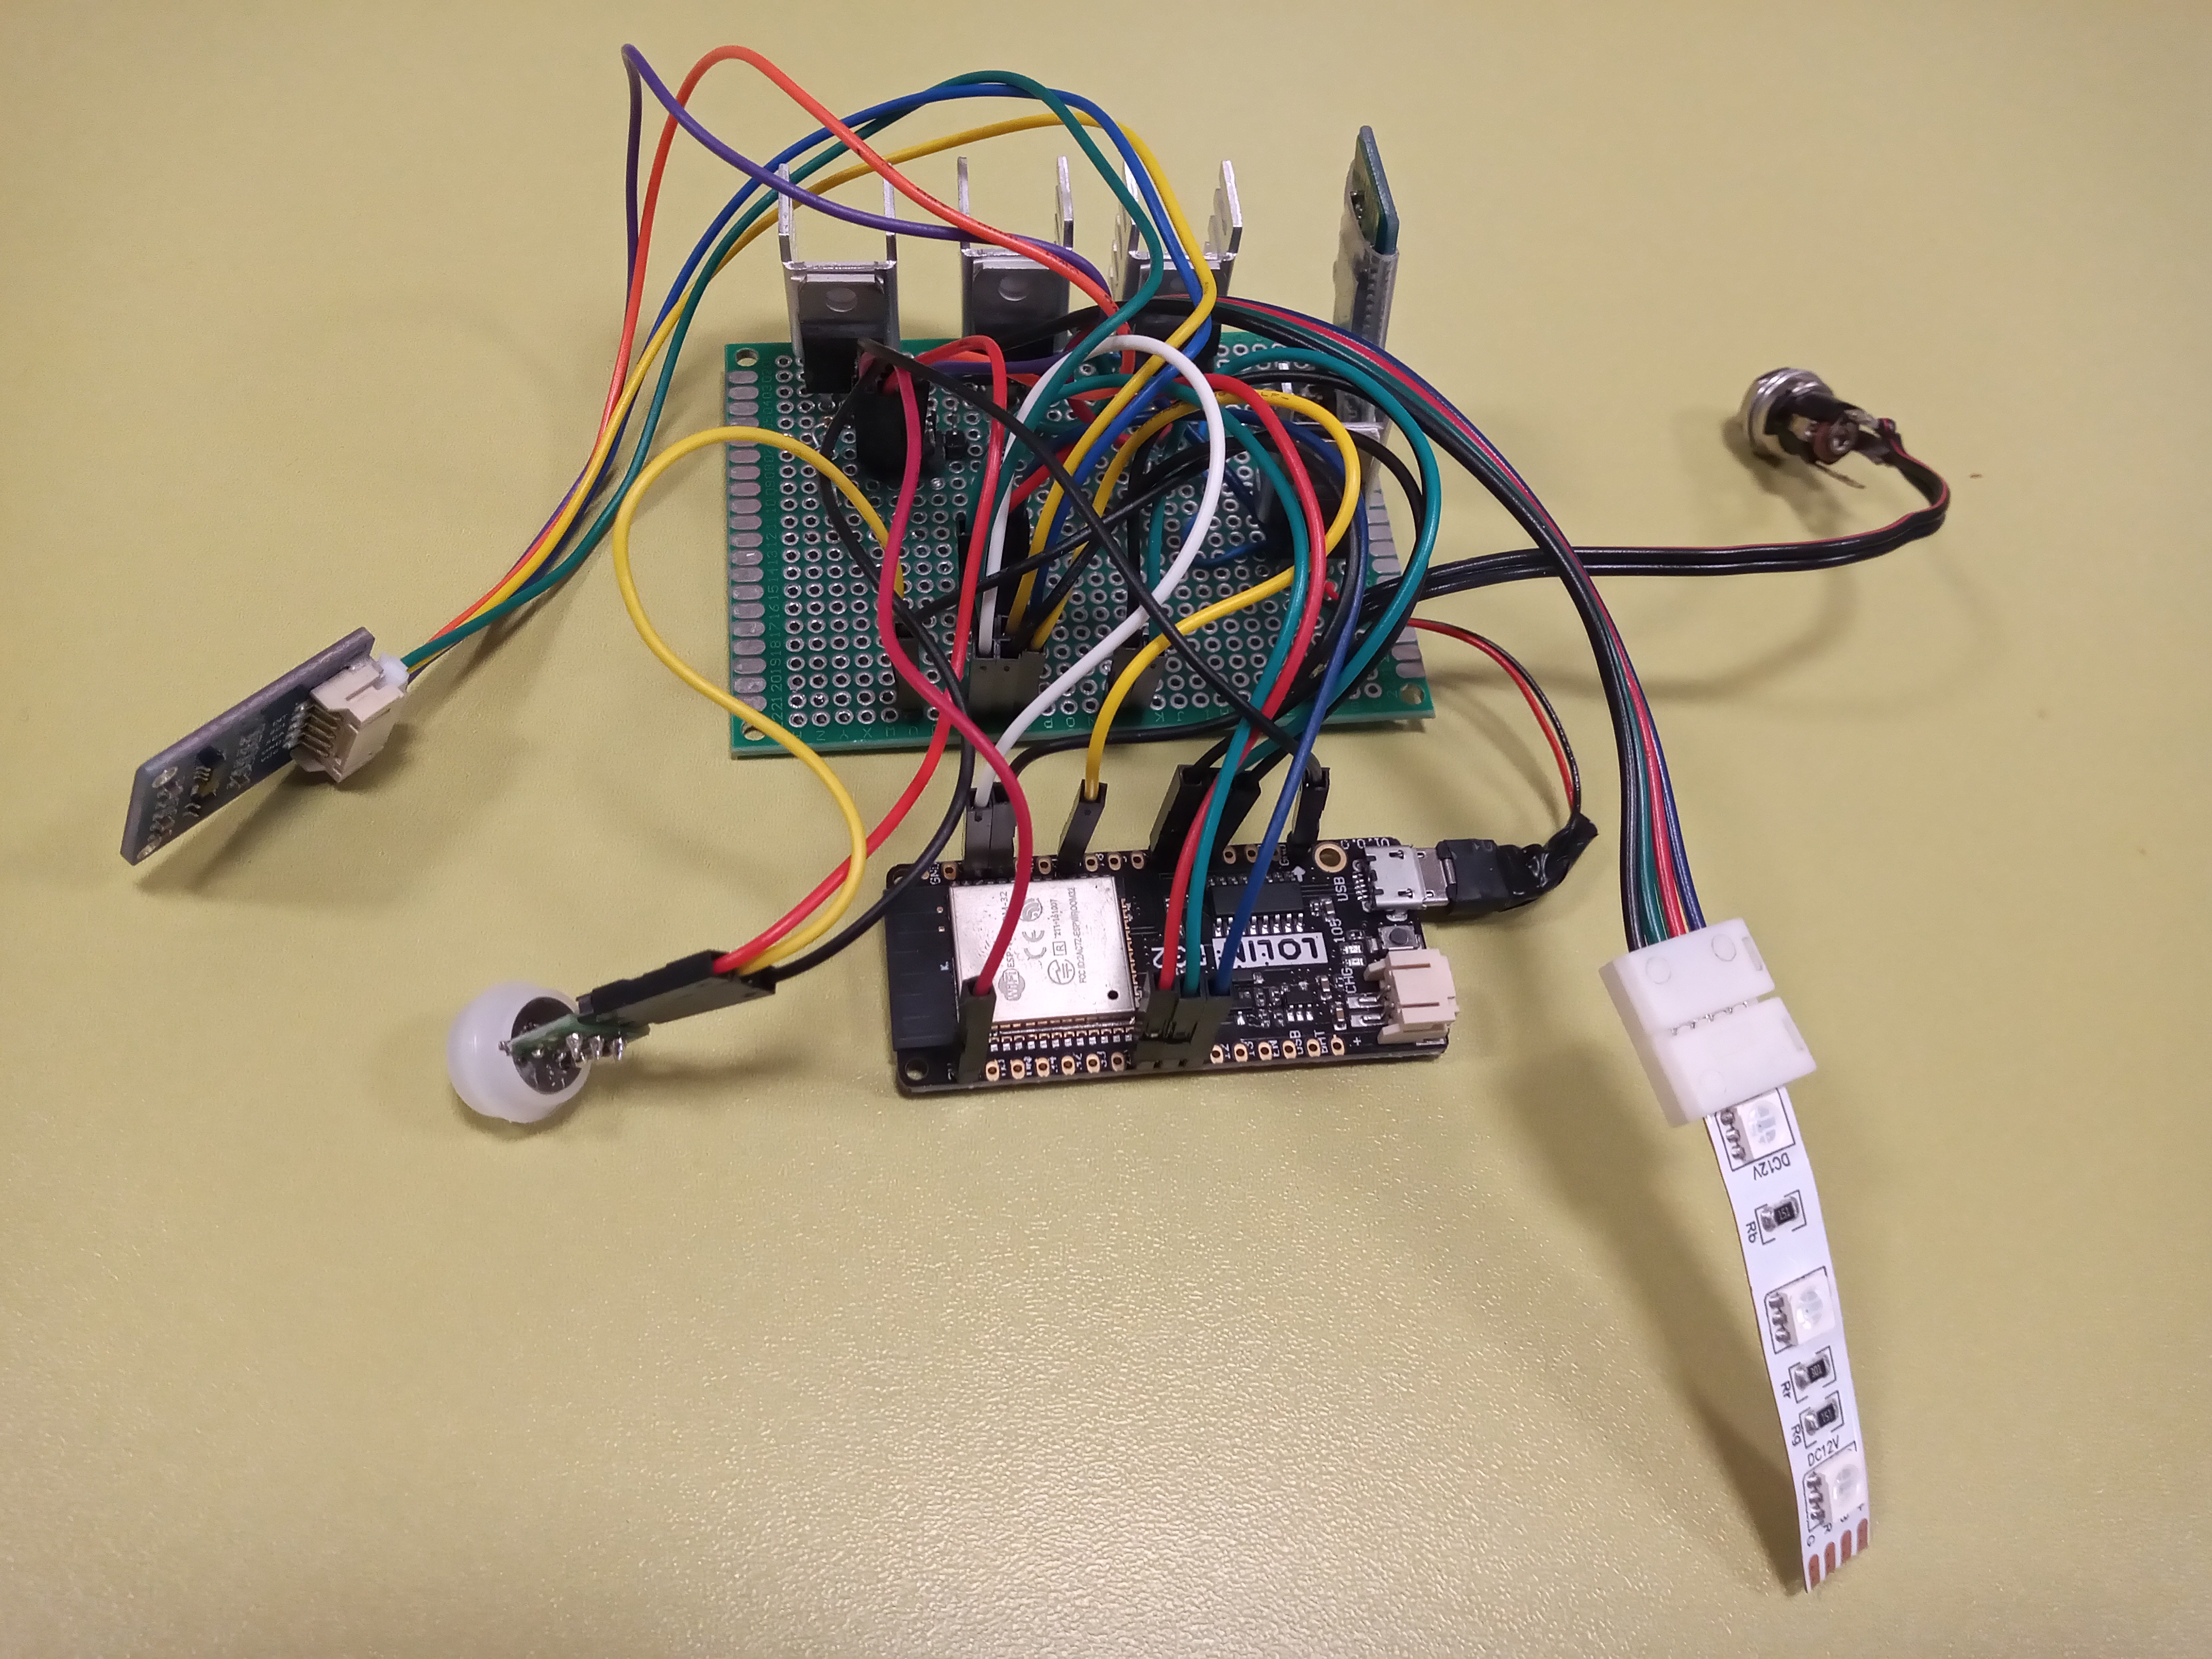
\includegraphics[width=\textwidth]{assets/prototype.jpg}
\end{subfigure}
\hfill
\begin{subfigure}[h]{0.48\textwidth}
	\centering
	\includegraphics[width=\textwidth]{assets/prototype-back.jpg}
\end{subfigure}
\caption{Plošný spoj kontroléra inteligentného svietidla}
\label{fig:pcb}
\end{figure}

\begin{figure}[h]
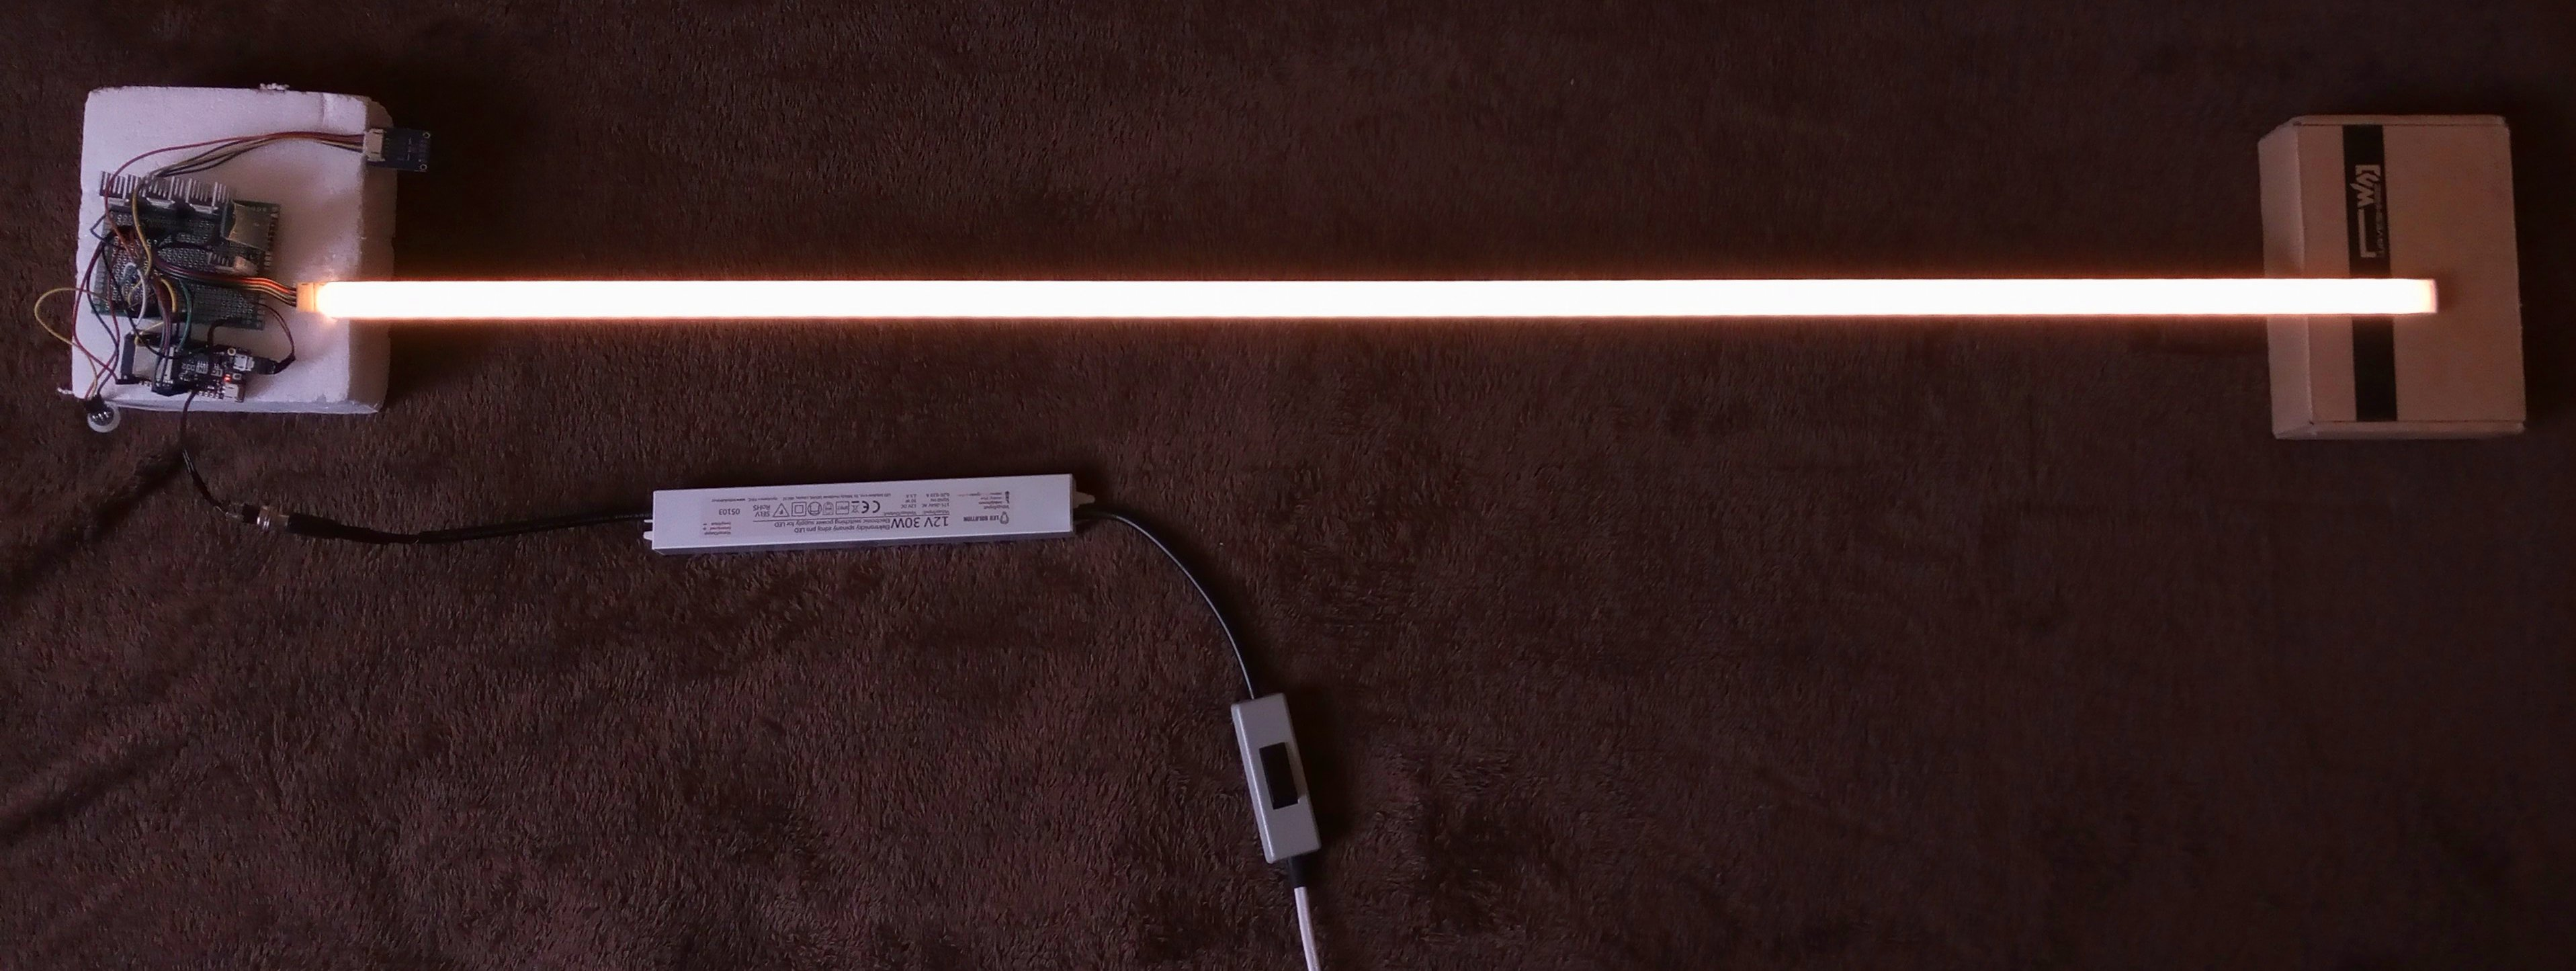
\includegraphics[width=\textwidth]{assets/lamp.jpg}
\caption{LED pásik namontovaný do metrovej hliníkovej lišty}
\label{fig:lamp-full}
\end{figure}


\textbf{Fimvér} pre zariadenie kontroléra LED pásika na ESP32 je napísaný v jazyku C za použitia SDK \textbf{ESP-IDF} (Espressif IoT Development Framework) vo verzii 5.0 \cite{noauthor_esp-idf_nodate}. Ako vývojové prostredie sme použili \emph{Visual Studio Code} a na zostavovanie a flashovanie programu slúži nástroj príkazového riadku \emph{idf.py}.

Obsluhu činností ako sú napr. príjem príkazov cez Bluetooth alebo obsluha prerušenia od detektora pohybu zabezpečujú úlohy operačného systému \emph{FreeRTOS}. Ovládače na bežné periférie ako sú: GPIO, PWM, Timer, UART, I2C, Non-volatile storage pochádzajú z SDK. Driver pre senzor osvetlenia od výrobcu pre vývojový platformu Arduino IDE je prepísaný a prispôsobený ku ESP-IDF.

\begin{lstlisting}[style=cstyle,caption=Štruktúra vlastností svietidla,label={lst:light-settings}]
typedef struct {
   bool status;
   bool movement;
   uint8_t brightness;
   uint16_t temperature;
   uint16_t threshold;
} Light;
\end{lstlisting}
Aktívny stav svietidla je uložený v štruktúre \verb|Light|, z ktorej existuje jedna globálna inštancia a prístup k nej je obmedzený cez mutex.

V hlavnom programe sa najprv načítajú nastavenia svetla od posledného vypnutia z nevolatilnej pamäte. Hoc by tento krok zlyhal použijú sa predvolené parametre (továrenské nastavenia). Ďalej sa nastaví interval pre časovač PIR senzora a obsluha prerušenia pri dosiahnutí času alarmu \emph{switch\_isr\_handler}, ktorá dokáže notifikovať úlohu na vypnutie svetla \emph{light\_switch\_task}.

Z periférii je potrebné nastaviť zbernice pre komunikáciu so senzorom osvetlenia, Bluetooth modulom a nakoniec sa LED diódy uvedú do stavu podľa načítaných nastavení. Systém spúšťa tri úlohy, ktoré prevažne blokujú pri čakaní na udalosti, buď na požiadavku o zmenu stavu svetla alebo o asynchrónny príjem príkazov na UART zbernici.

\begin{lstlisting}[style=cstyle,caption=Inicializácia hardvéru a spustenie úloh,label={lst:firmware-main},
morekeywords={xTaskCreate,xSemaphoreCreateMutex,timer_on_alarm,switch_isr_handler,light_switch_task,receive_commands_task}]
void app_main(void)
{
   light_mutex = xSemaphoreCreateMutex();
   lux_sensor_mutex = xSemaphoreCreateMutex();

   nvs_config(); 
   nvs_load(&light);
   timer_setup(&timer, PIR_TIMEOUT_S, timer_on_alarm);
   pir_sensor_config(switch_isr_handler);
   i2c_config();
   light_sensor_config();
   bluetooth_config();

	led_config();
   movement_detection(light.movement, timer,  timer_on_alarm, switch_isr_handler);
   uint16_t lux = illuminance_level();
   lamp_scene(lux); 

   xTaskCreate(light_switch_task, "detect_movement", 2048, (void *)true, 1, &gpio_task);
   xTaskCreate(light_switch_task, "timeout_light", 2048, (void *)false, 1, &timer_task);
   xTaskCreate(receive_commands_task, "receive_commands", 4096, NULL, 10, NULL);
}
\end{lstlisting}

\textbf{Softvér mobilnej aplikácie} je implementovaný v jazyku Kotlin vo vývojovom prostredí Android Studio v2022.1.1. Aplikácia podporuje ADK minimálne verzie 24, ale je zostavená a testovaná výhradne na smartfóne Motorola Moto E6 Plus s Android 9. Dizajn obrazovky je realizovaný podľa návrhu (Obr. \ref{fig:mobile-app}). Pri spustení akejkoľvek akcie sa overuje otvorené spojenie so svietidlom. Pokiaľ je dočasne nedostupné, dialógové okno zablokuje činnosť pre používateľa a snaží sa obnoviť Bluetooth pripojenie.

\begin{figure}[h]
\centering
\begin{subfigure}[b]{0.45\textwidth}
	\centering
	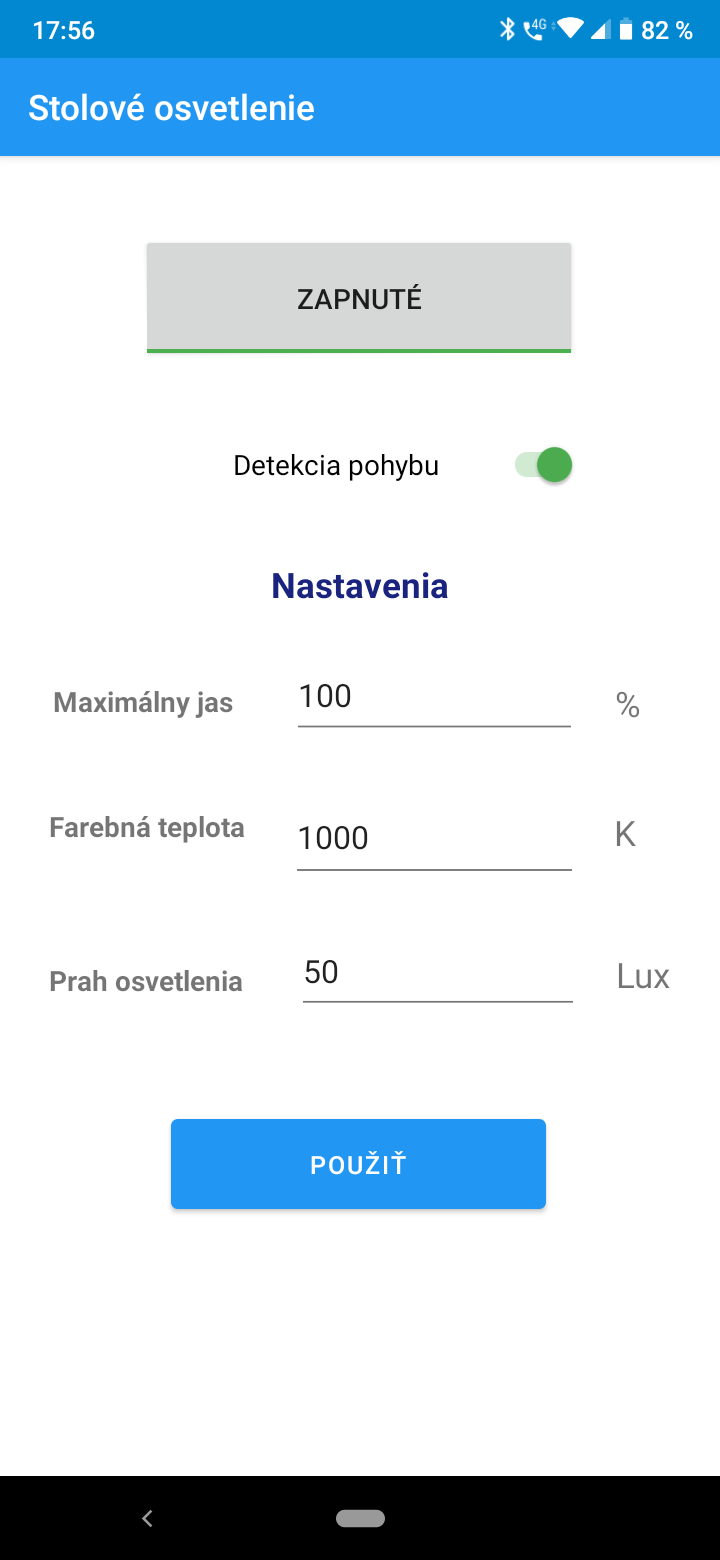
\includegraphics[width=\textwidth]{assets/mobile-app.png}
\end{subfigure}
\hfill
\begin{subfigure}[b]{0.45\textwidth}
	\centering
	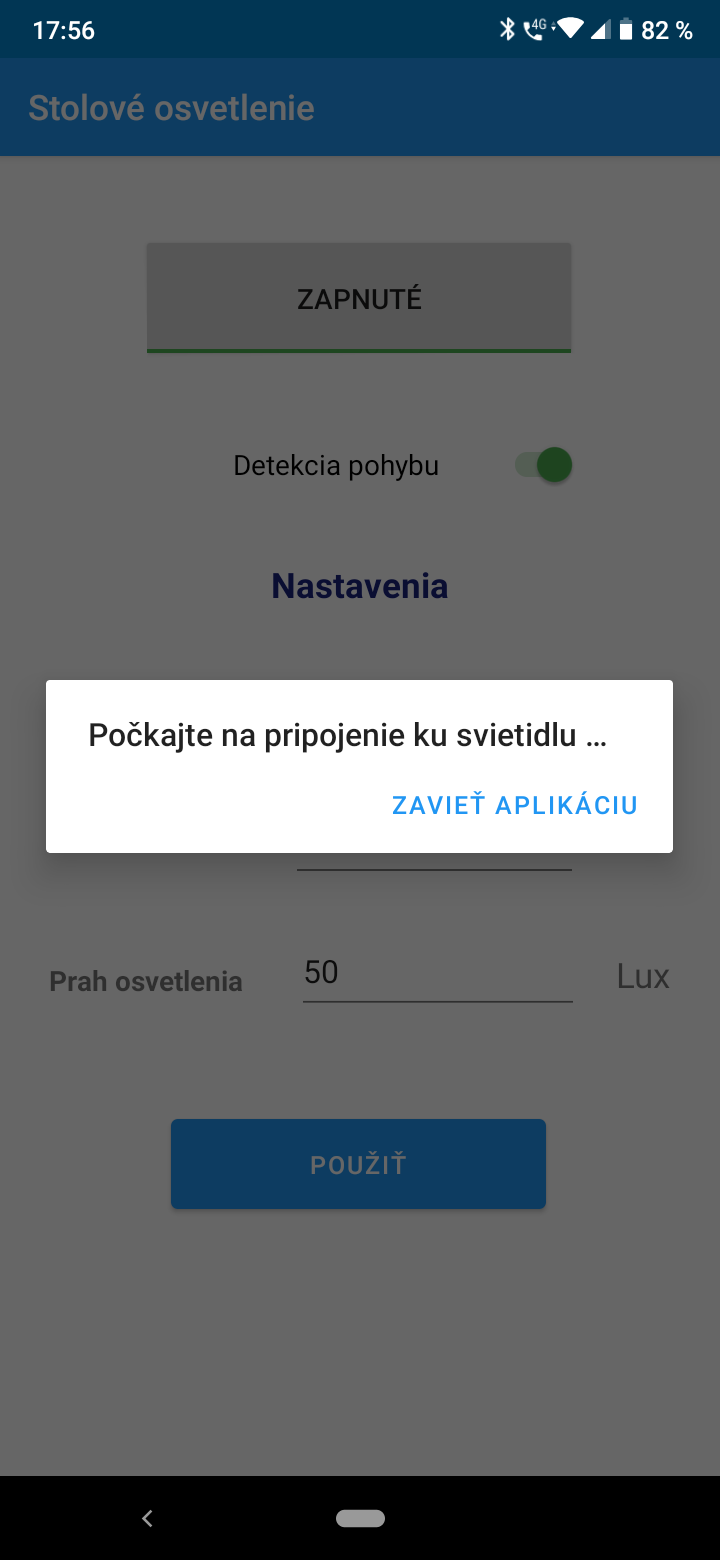
\includegraphics[width=\textwidth]{assets/mobile-app-connect.png}
\end{subfigure}
\caption{Obrazovka mobilnej aplikácie}
\label{fig:mobile-app}
\end{figure}


\section{Otestovanie riešenia}
Z dôvodu integrácie viacerých prvkov a konečnej použiteľnosti sme systém testovali cez \textbf{akceptačné testy}, ktoré definujú očakávané správanie z pohľadu používateľa. Vnorený systém prešiel všetkými uvedenými testami.
\vspace{1em}

\subsection{Test: Opakované nadväzovanie Bluetooth spojenia}
\noindent\textbf{Vstupné podmienky:} Mobilná aplikácia ani lampa nie sú spustené. Bluetooth na smartfóne je vypnutý, ale HC-05 je už spárované. \\
\textbf{Výstupné podmienky:} Mobilná aplikácia zobrazuje nastavenia svetla. \\
\textbf{Postup:}
\begin{enumerate}
\itemsep0pt
\item Používateľ otvorí aplikáciu s názvom ,,Stolové osvetlenie'' na svojom Android smartfóne
\item Aplikácia sa otvorí a zobrazí sa dialógové okno s vyžiadaním povolenia na aktivovanie Bluetooth.
\item Používateľ stlačí tlačidlo ,,Povoliť''.
\item Aplikácia vypíše v dialǵovom okne ,,Zapína sa rozhranie Bluetooth ...'', následne sa v smartfóne aktivuje Bluetooth. Aplikácia vypíše v dialógovom okne ,,Počkajte na pripojenie ku svietidlu ...'' a neumožňuje zrušenie tohto dialógového okna.
\item Používateľ pripojí lampu do elektrickej zásuvky a prepne prepínač lampy do polohy zapnuté.
\item Aplikácia maximálne do 15 sekúnd zatvorí dialógové okno a placeholders (vyšedené písmo) v textových poliach zmení za skutočné hodnoty (nevyšedené písmo).
\item Používateľ prepne prepínač lampy do polohy vypnuté a v mobilnej aplikácii klikne na ľubovoľné tlačidlo.
\item Aplikácie vypíše v dialógovom okne ,,Počkajte na pripojenie ku svietidlu ...'' a neumožňuje zrušenie dialógového okna.
\item Používateľ prepne prepínač lampy do polohy zapnuté.
\item Aplikácia znova maximálne do 15 sekund zatvorí dialógové okno a placeholders (vyšedené písmo) v textových poliach zmení za skutočné hodnoty (nevyšedené písmo).
\end{enumerate}

\subsection{Test: Aktívna detekcia pohybu}
\noindent\textbf{Vstupné podmienky:} Bluetooth spojenie aplikácie a lampy je nadviazané. Senzor osvetlenia je úplne zatmavený. Detekcia pohybu je podľa prepínača v aplikácii vypnutá. Svetlo je vypnuté, aj podľa tlačidla v aplikácii, aj fyzicky. \\
\textbf{Výstupné podmienky:} Svetlo je vypnuté, aj podľa tlačidla v aplikácii, aj fyzicky. \\
\textbf{Postup:}
\begin{enumerate}
\itemsep0pt
\item Používateľ stačí v aplikácii prepínač na zapnutie detekcie pohybu.
\item Aplikácia indikuje zmenou stavu prepínača v aplikácii, že detekcia pohybu je zapnutá.
\item Používateľ pohne rukou vo vzdialenosti 1 m na priamu viditeľnosť od stredu šošovky PIR senzora.
\item Svetlo sa zapne, aj podľa tlačidla v aplikácii, aj fyzicky.
\item Používateľ počká bez akéhokoľvek okolitého pohybu po interval nastavený vo firmvéri, predvolene 20 s.
\item Svetlo sa po 20 s samočinne vypne, aj podľa tlačidla v aplikácii, aj fyzicky.
\end{enumerate}

\subsection{Test: Deaktivovaná detekcia pohybu}
\noindent\textbf{Vstupné podmienky:} Bluetooth spojenie aplikácie a lampy je nadviazané. Senzor osvetlenia je úplne zatmavený. Detekcia pohybu je podľa prepínača v aplikácii vypnutá. Svetlo je vypnuté. \\
\textbf{Výstupné podmienky:} Svetlo je vypnuté, aj podľa tlačidla v aplikácii, aj fyzicky. \\
\textbf{Postup:}
\begin{enumerate}
\itemsep0pt
\item Používateľ pohne rukou vo vzdialenosti 1 m na priamu viditeľnosť od stredu šošovky PIR senzora.
\item Svetlo zostane vypnuté.
\end{enumerate}

\subsection{Test: Manuálne zapnutie a vypnutie svetla}
\noindent\textbf{Vstupné podmienky:} Bluetooth spojenie aplikácie a lampy je nadviazané. Senzor osvetlenia je úplne zatmavený. Detekcia pohybu je podľa prepínača v aplikácii zapnutá, jas je 100\%. Svetlo je vypnuté, aj podľa tlačidla v aplikácii, aj fyzicky. \\
\textbf{Výstupné podmienky:} Svetlo je vypnuté, aj podľa tlačidla v aplikácii, aj fyzicky. \\
\textbf{Postup:}
\begin{enumerate}
\itemsep0pt
\item Používateľ stačí v aplikácii prepínač na vypnutie detekcie pohybu.
\item Aplikácia indikuje zmenou stavu prepínača v aplikácii, že detekcia pohybu je vypnutá.
\item Používateľ stačí v aplikácii tlačidlo ,,Vypnuté''.
\item Svetlo sa zapne, aj podľa tlačidla v aplikácii, aj fyzicky.
\item Používateľ počká po interval nastavený vo firmvéri, predvolene min. 20 s.
\item Svetlo zostane zapnuté, aj po 30 s.
\item Používateľ stačí v aplikácii tlačidlo ,,Zapnuté''.
\item Svetlo je vypnuté.
\end{enumerate}

\subsection{Test: Zmena farebnej teploty svetla}
\noindent\textbf{Vstupné podmienky:} Bluetooth spojenie aplikácie a lampy je nadviazané. Senzor osvetlenia je úplne zatmavený. Svetlo je vypnuté, detekcia pohybu je vypnutá, jas je 100~\%, farebná teplota je 3000~K. \\
\textbf{Výstupné podmienky:} Svetlo je zapnuté a svieti jasným bielym svetlom. \\
\textbf{Postup:}
\begin{enumerate}
\itemsep0pt
\item Používateľ zadá do textového poľa ,,Farebná teplota'' hodnotu ,,1000'' a stlačí tlačidlo ,,Použiť''.
\item Aplikácia akceptuje vstup a odošle farebnú teplotu cez Bluetooth na lampu.
\item Používateľ stačí v aplikácii tlačidlo ,,Vypnuté''.
\item Svetlo sa zapne a svieti oranžovou farbou.
\item Používateľ zadá do textového poľa ,,Farebná teplota'' hodnotu ,,5000'' a stlačí tlačidlo ,,Použiť''.
\item Aplikácia akceptuje vstup a svetlo zmení farbu na bielu.
\end{enumerate}

\subsection{Test: Zmena jasu svetla}
\noindent\textbf{Vstupné podmienky:} Bluetooth spojenie aplikácie a lampy je nadviazané. Senzor osvetlenia je úplne zatmavený. Svetlo je vypnuté, detekcia pohybu je vypnutá, jas je 100\%, farebná teplota je 3000~K. \\
\textbf{Výstupné podmienky:} Svetlo je zapnuté a svieti jasným bielym svetlom. \\
\textbf{Postup:}
\begin{enumerate}
\itemsep0pt
\item Používateľ zadá do textového poľa ,,Maximálny jas'' hodnotu ,,10'' a stlačí tlačidlo ,,Použiť''.
\item Aplikácia akceptuje vstup a odošle jas cez Bluetooth na lampu.
\item Používateľ stačí v aplikácii tlačidlo ,,Vypnuté''.
\item Svetlo sa zapne a svieti bielou farbou slabej intenzity.
\item Používateľ zadá do textového poľa ,,Maximálny jas'' hodnotu ,,0''' a stlačí tlačidlo ,,Použiť''.
\item Svetlo je zapnuté, ale nesvieti.
\item Používateľ zadá do textového poľa ,,Maximálny jas'' hodnotu ,,100''' a stlačí tlačidlo ,,Použiť''.
\item Svetlo sveti bielou farbou silnej intenzity.
\end{enumerate}

\subsection{Test: Reakcia svetla na okolité osvetlenie}
\noindent\textbf{Vstupné podmienky:} Bluetooth spojenie aplikácie a lampy je nadviazané. Senzor osvetlenia odkrytý a zo vzdialenosti 10 cm svieti naň ,,Baterka'' zo smartfónu. Svetlo je vypnuté, detekcia pohybu je vypnutá, intenzita je 100\%.
\textbf{Výstupné podmienky:} Svetlo je zapnuté. \\
\textbf{Postup:}
\begin{enumerate}
\itemsep0pt
\item Používateľ zadá do textového poľa ,,Prah osvetlenia'' hodnotu ,,10'' a stlačí tlačidlo ,,Použiť''.
\item Aplikácia akceptuje vstup a odošle prahovú hodnotu cez Bluetooth na lampu.
\item Používateľ stačí v aplikácii tlačidlo ,,Vypnuté'', to zmení nápis na ,,Zapnuté''.
\item Svetlo sa nezapne a text tlačidla sa vráti naspäť na ,,Vypnuté''
\item Senzor osvetlenia je zatmavený a prestane naň svietiť ,,Baterka''. Používateľ stačí v aplikácii tlačidlo ,,Vypnuté'', to zmení nápis na ,,Zapnuté''.
\item Svetlo sa zapne.
\end{enumerate}

\subsection{Test: Načítanie pôvodných nastavení po zapnutí}
\noindent\textbf{Vstupné podmienky:} Bluetooth spojenie aplikácie a lampy je nadviazané. Senzor osvetlenia je úplne zatmavený. Svetlo je zapnuté, detekcia pohybu je vypnutá.
\textbf{Výstupné podmienky:} Svetlo je vypnuté, detekcia pohybu je vypnutá, jas je 100\%, farebná teplota je 5000 K, prah je 1000. \\
\textbf{Postup:}
\begin{enumerate}
\itemsep0pt
\item Používateľ zadá do textového polí hodnoty: ,Farebná teplota'' = ,,5000'', ,,Maximálny jas'' = ,,100'',  ,,Prah osvetlenia'' = ,,1000'' a stlačí tlačidlo ,,Použiť''.
\item Aplikácia akceptuje vstup a odošle hodnoty cez Bluetooth na lampu.
\item Svetlo sa bude mať vlastnosti podľa zmenených nastavení.
\item Používateľ stačí v aplikácii tlačidlo ,,Zapnuté'', to zmení nápis na ,,Vypnuté''.
\item Svetlo sa vypne.
\item Používateľ prepne prepínač lampy do polohy vypnuté a zatvorí mobilnú aplikáciu, počká na zhasnutie indikačnej ledky na MCU.
\item Používateľ prepne prepínač lampy do polohy zapnuté a otvorí mobilnú aplikáciu.
\item Aplikácia sa pripojí na lampu cez Bluetooth a načíta posledné uložené nastavenia.
\item Používateľ stačí v aplikácii tlačidlo ,,Vypnuté''.
\item Fyzické vlastnosti svetla budú rovnaké ako pred vypnutím.
\end{enumerate}

\section{Zhodnotenie výsledkov}
V semestrálnom projekte sme vytvorili vnorený systém postavený na vývojovej doske ESP32 Lolin D32, podľa zadania a špecifikácie požiadaviek. Zariadenie ovláda nastavenia RGB LED pásiku podľa vstupov od PIR senzora pohyba, senzora vonkajšieho osvetlenia, a príkazov z mobilnej aplikácie na platforme Android komunikujúcej cez Bluetooth RFCOMM s modulom HC-05.

Na základe analýzy dostupnej ponuky vhodných typov senzorov a LED osvetlenia sme navrhli systém na spínanie stolnej lampy, pričom sme museli vyriešiť distribúciu viacerých napájacích napätí pre prvky v systéme, pripojenie a komunikáciu so senzormi cez mikroprocesorové zbernice, a scenáre spínania svetla. Firmvér je implementovaný v jazyku C v SDK ESP-IDF. Mobilná aplikácia je napísaná v jazyku Kotlin a jej hlavnou úlohou je posielanie Bluetooth príkazov zariadeniu.

Správnosť systému ako celku sme overili sériou akceptačných testov s kladnými výsledkami pri každom z nich. Použitie RGB svetiel umožňuje rozšírenie do budúcna pre ďalšie farebné scény.

\printbibliography[title={Zoznam použitej literatúry}]

\section{Technická dokumentácia}
\subsection{Prehľad hardvérových súčiastok}
Na základe predošlej analýzy sme zostavili zoznam súčiastok potrebných pre zhotovenie zariadenia. Cena hardvéru prototypu (jednokusová výroba) je odhadovaná na 55 \texteuro, na základe nami zvolených dodávateľov.

\paragraph{Riadiaca jednotka}
\begin{itemize}
\itemsep0pt
\item ESP32 WeMos Lolin D32 - Mikrokontrolér
\item HC-05 - Bluetooth modul
\end{itemize}

\paragraph{Senzory a akčné členy}
\begin{itemize}
\itemsep0pt
\item RGB LED pásik 14,4W/m 12V bez krytia IP20 1m
\item Olimex PIR-SB312 10x8mm
\item WS-17146 TSL25911 Light Sensor
\end{itemize}

\paragraph{Elektrické súčiastky}
\begin{itemize}
\itemsep0pt
\item L7805CV Lineárny regulátor napätia 12V na 5V
\item NPN Tranzistor BD711
\item Rezistory - 220 $\Omega$, 330 $\Omega$
\item LED zdroj (trafo) 12V 30W IP67
\item Flexo šnúra – 3m
\item Konektory: RGB LED pásik, Micro USB-B, DC konektor a zásuvka
\end{itemize}

\paragraph{Mechanické súčiastky}
\begin{itemize}
\itemsep0pt
\item DO1 chladič
\item DO3A chladič
\item Univerzálny plošný spoj
\item Nástenný profil N3 biely, Opálový kryt 1m
\item Koncovka profilu N3 biela
\item Vypínač mezišnúrový
\end{itemize}

\subsection{Zdrojové súbory pre firmvér}
Implementácia firmvéru sa nachádza v priečinku \emph{esp}. Na nahratie firmvéru na MCU je potrebné mať stiahnuté a nainštalované ESP-IDF s požadovanými systémovými závislosťami podľa dokumentácie. Potom vykonáme v priečinku \emph{esp} tieto príkazy:
\begin{verbatim}
source /path/to/esp-idf/export.sh
idf.py build
idf.py -p /dev/ttyUSB0 flash
\end{verbatim}

Firmvér je rozdelený do viacerých súborov zdrojového kódu obsahujúce popísanú funkcionalitu:
\begin{itemize}
\itemsep0pt
\item \textbf{main.c} - Hlavný program, úlohy a obsluhy prerušení.
\item \textbf{storage.c} - Načítanie a zapis nastavení svetla z/do nevolatilnej pamäte.
\item \textbf{trigger.c} - Nastavenie časovača a prerušení po timeout a pri detekcii pohybu.
\item \textbf{i2c.c} - Zjednodušenie rozhrania pre komunikáciu cez I2C zbernicu.
\item \textbf{lightsensor.c} - Ovládač pre senzor osvetlenia. Externe prístupné sú iba funkcie \emph{light\_sensor\_config()}, \emph{light\_sensor\_read\_lux()}
\item \textbf{bluetooth.c} - Inicializácia UART linky na príslušných pinoch \emph{bluetooth\_config()}, parsovanie príkazov v prijatej správe na ovládanie svetla \emph{parse\_commands()} a odoslanie aktuálneho stavu lampy \emph{bluetooth\_send\_status()}
\item \textbf{led.c} - Konfigurácia PWM kanálov \emph{led\_config()} a nastavenie LED diód podľa rôznych parametrov, buď cez priamo požadovanú RGB farbu \emph{led\_set\_color()} alebo s prepočtom z farby a jasu  \emph{led\_output()}.
\end{itemize}

\subsection{Zdrojové súbory pre Android aplikáciu}
Zdrojový kód mobilnej aplikácie a nastavenia vývojového prostredia sa nachádzajú v priečinku \emph{led-light-app}, s rozmiestnením súborov podľa predvolenej štruktúry z Android Studio. Hlavná aktivita sa nachádza v súbore \emph{MainActivity.kt} vnúri \emph{app/src/main/java/com/smartdevice/tablelantern/}. Rozmiestnuje UI prvky na obrazovke,
iniciuje a prijíma správy od Bluetooth služby v \emph{BluetoothService.kt}.

V triedach prítomných v aplikácii sa nachádzajú tieto najdôležitejšie metódy:
\paragraph{class MainActivity}
\begin{itemize}
\itemsep0pt
\item \verb|onCreate()| - vytvorenie UI komponentov a inicializácia Bluetooth služby (\emph{BluetoothService}).
\item \verb|onSwitchLight()| - Udalosť tlačidla na odoslanie príkazu cez Bluetooth na zmenenie stavu svetla.
\item \verb|onMotionDetectSwitch()| -  Udalosť tlačidla na odoslanie príkazu cez Bluetooth na (de)aktiváciu detektora pohybu.
\item \verb|onApplySettings()| - Udalosť tlačidla na odoslanie želaných nastavení svetla s ich validáciou.
\item \verb|lampConnect()| - Nájdenie modulu HC-05 medzi spárovanými zariadeniami a otvorenie Bluetooth spojenia, na ten účel volá metódu \verb|BluetoothService.connect()|
\item \verb|setLightState()| - Spätné volanie (callback) po prijatí konfigurácie od vnoreného systému na jej parsovanie a načítanie do textových polí v aplikácii.
\item \verb|BlHandler.handleMessage()| - Zobrazovanie správ z Bluetooth služby v UI rozhraní.
\end{itemize}

\paragraph{class BluetoothService}
\begin{itemize}
\itemsep0pt
\item \verb|connect()| - Spúšta vlákno \emph{ConnectThread}. Slúži ako rozhranie pre \emph{MainActivity} na prístup k vnútorným triedam vlákien.
\item \verb|connected()| - Spúšta vlákno \emph{ConnectThread}. Slúži ako rozhranie pre \emph{MainActivity} na prístup k vnútorným triedam vlákien.
\item \verb|send()| - Služí ako rozhranie voči \emph{MainActivity} a volá \emph{ConnectedThread.write()} so argumentmi v správnom formáte.
\item \verb|ConnectThread.run()| - Hlavná metóda vlákna \emph{ConnectThread} na nadviazanie Bluetooth spojenia cez RFCOMM socket. Volá metódu \emph{connected}.
\item \verb|ConnectedThread.run()|  - Hlavná metóda vlákna \emph{ConnectedThread} čaká na príjem bajtov z otvoreného Bluetooth socket. Po prijatí celistvej správy stavu vnoreného systému notifikuje hlavnú aktivitu.
\item \verb|ConnectedThread.write()| - Metóda na odoslanie bajtov na zariadenie cez otvorený Bluetooth socket.
\end{itemize}


\subsection{Syntax Bluetooth príkazov}
Zariadenie lampy komunikuje cez Bluetooth RFCOMM prostredníctvom preddefinovanej sady textových príkazov. Príkazy posielané hneď za sebou musia byť oddelené ľudovoľným oddeľovačom napr. medzerou alebo čiarkou. Po poslaní aktivovaní konfiguračného príkazu sa ako odpoveď vráti aktuálny stav svetla vo formáte podľa príkazu \emph{REQ}.
\begin{itemize}
\item \textbf{SWITCH} - Prepnutie aktuálneho stavu svetla. Ak je zapnuté, tak sa vypne a naopak.
\item \textbf{DETECT} - Prepnutie aktualnej aktívnosti detektora pohybu.
\item \textbf{LEVEL [level]} - Jas svetla v percentách z celkovej svietivosti. Validná hodnota pre parameter \emph{level} je celé číslo v rozsahu 0 - 100 vrátane.
\item \textbf{KELVIN [temp]} - Farebná teplota svetla v kelvinoch. Validná hodnota pre parameter \emph{temp} je celé číslo v rozsahu 1000 - 40000 vrátane.
\item \textbf{LUX [threshold]} - Prahová úroveň vonkajšieho osvetlenia v luxoch, pod ktorú sa svetlo rozsvieti. Validná hodnota pre parameter \emph{threshold} je celé číslo v rozsahu 0 - 10000 vrátane. Nepredpokladá sa zapínanie svetla pri vysokej úrovni vonkajšieho osvetlenia.
\item \textbf{REQ} - Aktuálny stav svetla vo formáte: \emph{,,{S/0,M/0,K/2000,B/100,L/5}''}. Písmená označujú príslušné parametre takto: \textbf{S} - stav svetla (0 alebo 1), \textbf{M} - aktívnosť detektora pohybu  (0 alebo 1), \textbf{K} - farebná teplota, B - jas,  L - prahová úroveň osvetlenia. Rozsah hodnôt je rovnaký ako pri konfiguračných príkazov.
\end{itemize}

\end{document}

